\scanpage{86}
% archive foliation: 85
Soit $\mathcal T_\nu^!$ le ss-groupe de $\mathcal T_\nu$
formé des éléments qui satisfont
aux relations précédentes. Donc on a
\[
1\longrightarrow\mathcal T_\nu^{!0}\unsure{-|\longrightarrow}\mathcal T_\nu^!\longrightarrow\widehat{\mathbb Z}^{*}\unsure{-|\longrightarrow}1
\]
avec
\[
\begin{gathered}
\mathcal T_\nu^{!0}\subset\mathcal T_\nu^0\\
\text{''}\\
\{\gamma\in\mathcal T_\nu^0\mid\gamma\text{ commute aux }\rho_\nu(i)
\text{ et à }t_\nu\}
\end{gathered}
\]
\figure{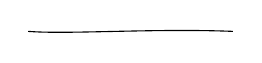
\begin{tikzpicture}\draw (0,0)..controls (.5,-.04) and (1.6,.04)..(2.6,0);\end{tikzpicture}}

Si $\nu=2$ il y a un autre choix
intéressant de $I_{\unsure{0}}\subset\mathbb P^1(\overline{\mathbb Q})$, savoir
\[
I=\{0,1,\infty\}\qquad(\text{plutôt que }I=\mu_3(\overline{\mathbb Q}))
\]
qui donne lieu à action de
$\unsure{\mathfrak S|\mathcal S}_3$ sur $(X_0/I_0/k)$ --- on trouve
action de $\Gamma\times\unsure{\mathfrak S|\mathcal S}_3$ sur $\unsure{F_2|\Gamma_2}^{\mathrm{ext}}$, i.e.
\[
\Gamma\times\unsure{\mathfrak S|\mathcal S}_3\longrightarrow\widetilde{\mathcal T}_2
\]
